\chapter{De la Señal Fotofísica al Observable Biológico}
\label{cap:MatMet}


En este capítulo, detallaré cómo analizar experimentos de microscopía de anisotropía en polarización de un biosensor como el utilizado por el grupo previamente en el trabajo de \cite{Stegemann2015}. Comenzaré por una descripción de la microscopía de anisotropía de polarización utilizada para observar este tipo de sensores, cómo transfectarlo a las células y el protocolo de adquisición y análisis de imágenes pertinente. Finalmente, a partir de un modelo minimalista que incluya estos biosensores, desarrollaré como estimar la actividad de cada caspasa a partir de los cambios en anisotropía del biosensor correspondiente y definiré un observable robusto que sirve de referencia a la activación de la caspasa.



%%%%%%%%%%%%%%%%%%%%%%%%%%%%%%%%
\section{Microscopía de Anisotropía de Polarización}


Los fluoróforos en particular poseen momentos de transición de absorción y emisión subtendidos en direcciones específicas. Esto se traduce en que la probabilidad de excitar un fluoróforo con luz linealmente polarizada depende del ángulo entre el eje de polarización de la excitación y el momento de transición de excitación y, a su vez, la emisión será polarizada y paralela al momento de transición de emisión. La polarización de la emisión puede ser afectada por diversos factores. Para empezar, los momentos de transición de excitación y emisión no siempre son colineales. Adicionalmente, el fluoróforo excitado puede rotar libremente durante el tiempo de vida del estado excitado contribuyendo así a la depolarización. Es así que cuando el tiempo de vida del estado excitado es mayor o comparable a la escala temporal de la difusión rotacional, dichos fluoróforos se implementan en biofísica para el análisis de viscosidad del medio en el que se encuentran inmersos \citep{Lakowicz2006}.

Debido a que ambos fluoróforos que componen un biosensor basado en homoFRET son indistinguibles espectralmente (como el de \cite{Stegemann2015}), necesitaremos hacer uso de otras propiedades de la luz para determinar su estado. En este caso, utilizaremos las propiedades depolarizantes del biosensor para estimar el estado de la población. Sabiendo que en el citoplasma celular el tiempo de vida de fluorescencia es considerablemente menor que el tiempo característico de rotación para una proteína fluorescente (y aún más para un dímero), ésta no contribuirá fuertemente a la depolarización. Sin embargo, la contribución a la depolarización debido a FRET es considerable ya que los fluoróforos aceptores se encuentran alineados aleatoriamente. De está forma, la población de biosensores en estado dimérico contribuirá más fuertemente a la depolarización que aquellos en estado monomérico.

Usualmente, la anisotropía se utiliza como medida de la polarización de una muestra. La anisotropía se define matemáticamente como

\begin{equation}
    r = \frac{I_{\parallel} - I_{\perp}}{I_{\parallel} + 2 I_{\perp}}.
    %\label{eq:anisotropia}
\end{equation}

\noindent Esto se consigue experimentalmente mediante el uso de analizadores para observar la intensidad de fluorescencia emitida en el eje paralelo al de incidencia (I$_{\parallel}$), así como también en el eje perpendicular (I$_{\perp}$). Cabe destacar que se trata de una magnitud adimensional ya que está normalizada por la intensidad total de fluorescencia y, por lo tanto, es independiente de la concentración de fluoróforo presente.

La anisotropía de una muestra puede medirse tanto en cubetas como mediante microscopía. La microscopía de fluorescencia permite indagar sobre las propiedades y el comportamiento de las células de forma poco invasiva y con elevada especificidad y sensibilidad. Considerando los componentes necesarios, resulta simple adaptar un microscopio comercial para visualizar anisotropía de polarización. En primer lugar, se debe colocar un polarizador en el camino del haz de excitación. Hay más de una forma de adaptar el canal de emisión para poder visualizar ambas polarizaciones simultáneamente o secuencialmente. Utilizando cristales birefringentes como calcita, es posible separar el haz en sus dos componentes de polarizaciones perpendiculares y utilizar tanto dos detectores como regiones separadas del sensor de una única cámara. Por otro lado, si la velocidad del sistema es considerablemente mayor que la variación de anisotropía de la muestra, se pueden colocar dos analizadores cruzados en una rueda de filtros para seleccionar la polarización a ser adquirida (ver \cref{fig:esquemaAnisotropia}).

\begin{figure}
    \centering
    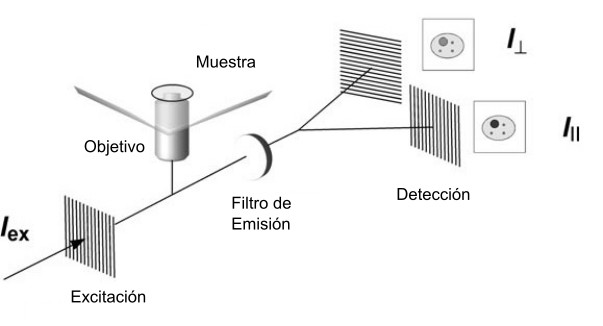
\includegraphics[width=0.75\textwidth]{img/cap_2/EsquemaAnisotropia.png}
    \caption{\footnotesize{Esquema de un armado experimental típico de un microscopio adaptado para ver anisotropía de polarización. Se utiliza un polarizador para que la excitación sea linealmente polarizada. El haz ingresa a la muestra y la fluorescencia es colectada a través del mismo objetivo. Se utilizan dos analizadores para observar las componentes emitidas paralela y perpendicular a la excitación.}}
    \label{fig:esquemaAnisotropia}
\end{figure}

Durante la calibración del sistema, es necesario considerar y corregir las depolarizaciones introducidas por el sistema óptico utilizado. Por ejemplo, la elevada amplitud numérica de las lentes objetivo utilizadas capturan una mezcla de polarizaciones distintas debido al cono de luz de emisión subtendido en un amplio ángulo sólido en el punto de muestreo. La calibración del factor G se utiliza para corregir las diferencias en sensibilidad del sistema para polarizaciones cruzadas. Para determinarlo, se utiliza un valor de referencia de anisotropía de un fluoróforo mediante la ecuación

\begin{equation}
    G = \frac{I_{\parallel} (1 - r_{ref})}{I_{\perp} (1 + 2r_{ref})},
\end{equation}

\noindent donde $r_{ref}$ es el valor de anisotropía conocido de la muestra. Dicho factor se utiliza en el cálculo de anisotropía siguiendo

\begin{equation}
    r = \frac{I_{\parallel} - G I_{\perp}}{I_{\parallel} + 2 G I_{\perp}}.
    % \label{eq:anisotropia}
\end{equation}

\noindent Al utilizar una referencia isótropa, como ser una muestra de fluoróforo diluido, es posible llegar a una expresión donde las intensidades paralela y perpendicular deben ser normalizadas por los valores de intensidad paralela y perpendicular medidas en la referencia. Esto tiene la doble ventaja de que al utilizar imágenes, se corrigen tanto inhomogeneidades en la iluminación como los factores depolarizantes del sistema óptico.


%%%%%%%%%%%%%%%%%%%%%%%%%%%%%%%%
\section{Diseño Experimental}


Para los experimentos descriptos en esta tesis, se utilizó un microscopio comercial invertido Olympus IX-81. Con el objetivo de adaptarlo se utilizaron tres polarizadores (Meadowlark Optics), uno de ellos en el camino de excitación, y dos de ellos en una rueda de filtros ubicada en el puerto lateral en el camino de emisión. Cabe destacar que se tuvo especial cuidado en la colocación del polarizador de excitación ya que debe estar alejado de fuentes de calor, como lo son algunas fuentes de iluminación. En este caso, la fuente de iluminación utilizada fue una MT20 de Olympus con una lámpara halógena conectada mediante fibra óptica de líquido. Se utilizó un objetivo HC PL APO 63x/1.4 NA CS2 de inmersión en aceite (Leica Microsystems). También fue utilizada una cámara Orca CCD (Hamamatsu Photonics). El software de adquisición consistió en CellR (Olympus).

El microscopio adaptado y utilizado se encuentra en el Instituto Max Planck de Fisiología Molecular de Dortmund, Alemania. Previo al inicio de la tesis doctoral, se desarrolló una rueda de filtros impresa en 3D y controlada por Arduino que actualmente es de libre acceso. Distintos modelos de estas ruedas fueron impresas para adaptar microscopios comerciales y un microscopio de iluminación de plano único (SPIM, por sus siglas en inglés) en nuestro laboratorio (\cref{fig:ruedas}).

\begin{figure}[b]
    \centering
    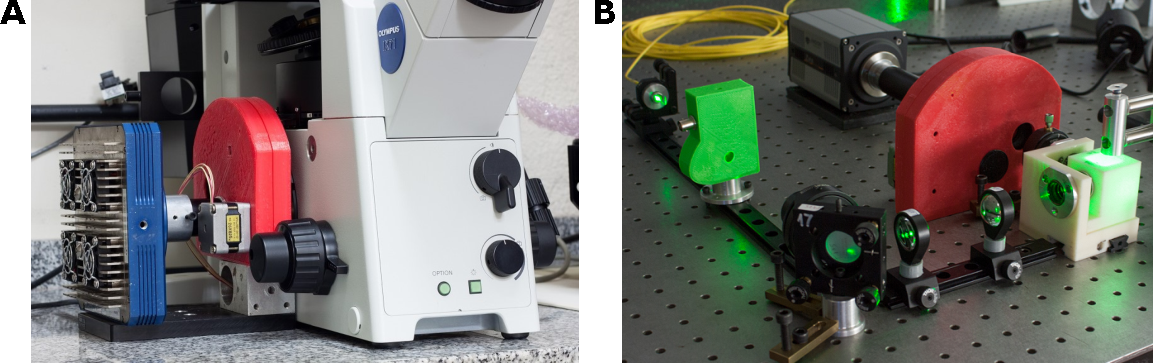
\includegraphics[width=0.9\textwidth]{img/cap_2/ruedas.pdf}
    \caption{\footnotesize{Imágenes de la rueda de filtros desarrollada en el laboratorio y montada en un microscopio comercial IX-71 (\textbf{A}) y uno de iluminación de plano único (\textbf{B}) para adaptarlos a microscopía de anisotropía de fluorescencia.}}
    \label{fig:ruedas}
\end{figure}

Las muestras consistían en células inmortalizadas de cáncer de cuello uterino (HeLa) cultivadas en pocillos de LabTek. Dado que es necesario mantenerlas viables a lo largo del experimento, las muestras se mantuvieron a 37$^{\circ}$C, 5\% de CO$_2$ y una humedad elevada $>$ 60\% mediante una cámara de cultivo y un Stable Z Specimen Warmer (Bioptechs Inc.). Dichas células fueron cultivadas en medio DMEM alto en glucosa, con 10\% de suero fetal bovino y suplementadas con 10~mg/ml de piruvato de sodio, 2~mmol/L de L-glutamina y antibióticos (100~U/mL penicilina, 100~$\mu$g/mL streptomicina) en una atmósfera humidificada, al 5\% de CO$_2$ y 37$^{\circ}$C.

Considerando que el proceso de apoptosis puede desencadenarse en cualquier momento entre el agregado de la droga estimulante y las 15 horas subsiguientes, fue necesario automatizar la adquisición de imágenes durante el experimento. Mediante una platina motorizada y el software CellR (Olympus) se programó el microscopio para adquirir imágenes secuenciales de varias posiciones de cada pocillo. En cada uno de los pocillos se colocaron distintas drogas que servían tanto de control como estímulo. Las imágenes adquiridas son posteriormente segmentadas y analizadas para generar un cuerpo de datos que contiene una curva de intensidad promedio en cada polarización y en cada célula detectada (\cref{fig:procedimiento_exp}).

\begin{figure}
    \centering
    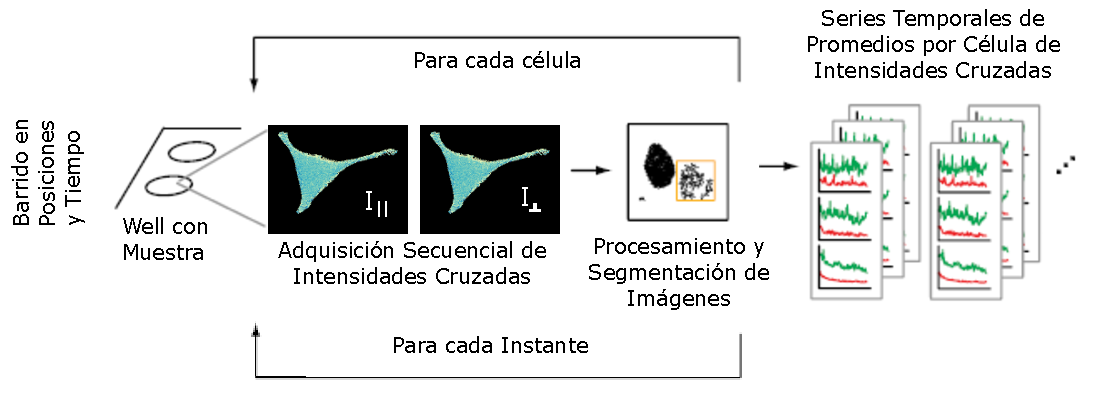
\includegraphics[width=0.7\textwidth]{img/cap_2/ProcedimientoExperimental.pdf}
    \caption{\footnotesize{Esquema del procedimiento experimental. Este consistió en sembrar las muestras con distintas drogas en pocillos de LabTek, adquirir una imagen de cada polarización en cada tiempo, segmentar y analizar dichas imágenes y, finalmente, generar un cuerpo de datos con las curvas de intensidad promedio de cada polarización de cada célula detectada.}}  
    \label{fig:procedimiento_exp}
\end{figure}

En cuanto a los parámetros de adquisición, se tuvieron varios cuidados distintos, tanto para no afectar significativamente la viabilidad de la muestra como para adquirir imágenes de suficiente calidad. Por un lado, la potencia de la iluminación no debe ser muy elevada ni prolongada para evitar el fotodaño a las células. Por otro lado, el tiempo de adquisición debe ser suficiente para aprovechar el rango dinámico de la cámara. Es importante destacar que no se debe buscar el 100 \% del rango dinámico ya que durante el transcurso del experimento la intensidad de fluorescencia por píxel va a aumentar y podría saturar por dos razones. En primer lugar, al clivarse el biosensor, su fluorescencia en el canal paralelo aumentará. En segundo lugar, las células al entrar en apoptosis se despegan del vidrio y adquieren una forma pequeña y redondeada que concentra el fluoróforo y aumenta la intensidad por píxel. La importancia de este cuidado radica, no solo en evitar saturar la región correspondiente a la célula imposibilitando su medición, sino que por efecto de arrastre de electrones se puede afectar la adquisición de toda la tira de píxeles, arruinando así otras regiones (\cref{fig:saturacion}). En el caso del sensor utilizado por el grupo previamente, se utilizó un tiempo de exposición de 50~ms y una potencia de iluminación elevada. Esto es posible ya que el fluoróforo implementado tiene una eficiencia cuántica elevada (0.74 según \cite{Griesbeck2001}) y su espectro de emisión se solapa con el rango de mayor eficiencia de detección de la cámara.

\begin{figure}[htb]
    \centering
    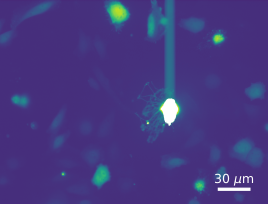
\includegraphics[width=0.35\textwidth]{img/cap_2/saturation.png}
    \caption{\footnotesize{Imagen de ejemplo de un grupo de células donde una de ellas aumentó tanto su intensidad que saturo la cámara y, además, ocurrió un arrastre de electrones a los otros píxeles de la tira afectando la adquisición.}}
    \label{fig:saturacion}
\end{figure}

Habiendo seleccionado los parámetros de adquisición, fue necesario elegir cuantas posiciones adquirir por pocillo. En resultados de análisis previos del grupo, Dr. Klaus Schuermann en Dortmund vio que las células tardaban entre 15 y 30 minutos en clivar su biosensor correspondiente. Por ello, se buscó llevar la resolución temporal de 10 minutos a mínimo 5 minutos y para esto se tuvo en cuenta el tiempo que se tarda en adquirir las imágenes correspondientes a cada polarización y la traslación de la platina motorizada. Cabe destacar que una vez adquirida la imagen, el microscopio tarda alrededor de 90~ms en cambiar de polarizador para adquirir la nueva imagen. Por otro lado, dependiendo la distancia entre las distintas posiciones, la platina tarda entre 1.3 y 2 segundos en trasladarse y entrar en foco (ver \cref{fig:tiempo_adq_un_canal}). El tiempo necesario para que la platina se traslade depende de la distancia entre posiciones, especialmente si esta debe trasladarse dentro de un mismo pocillo o entre pocillos. Dentro de los 5 minutos de resolución temporal, podemos adquirir múltiples posiciones ya que si demoramos como máximo 2 segundos en adquirir las imágenes correspondientes a una posición y trasladarnos a la siguiente, entonces seríamos capaces de adquirir 150 posiciones antes de volver a la primera. Finalmente, cada una de estas posiciones adquiridas suele contener entre 15 y 40 células, por lo que se estima adquirir 2250 a 6000 células por experimento. Una vez seleccionadas la máxima cantidad de posiciones posible de adquirir en menos de 5 minutos, se dejó el microscopio adquiriendo secuencialmente todas las imágenes a lo largo de las 15 horas del experimento. Utilizando una resolución temporal de 5 minutos durante 15 horas se adquieren 180 imágenes de una única polarización y posición, siendo 54000 imágenes en total.

\begin{figure}
    \centering
    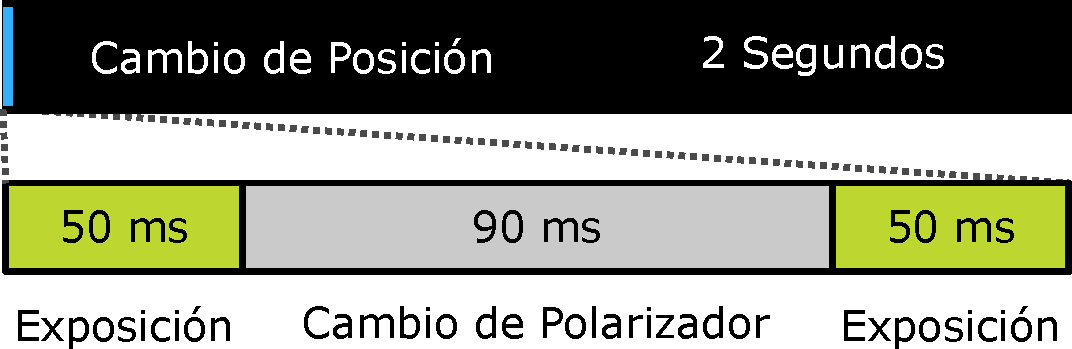
\includegraphics[width=0.5\textwidth]{img/cap_2/tiempo_adq_un_canal.pdf}
    \caption{\footnotesize{Esquema de los tiempos característicos de la adquisición secuencial de imágenes en cada polarización. En este caso se usaron 50 ms de tiempo de exposición para adquirir cada imagen, 90 ms entre cada polarización y 2 segundos para que la platina motorizada cambie de posición y entre en foco. El tiempo necesario para cambiar la configuración de polarizadores está incluido en el tiempo necesario para que la platina se traslade de una posición a otra.}}
    \label{fig:tiempo_adq_un_canal}
\end{figure}


%%%%%%%%%%%%%%%%%%%%%%%%%%%%%%%%%%%%
\section{Análisis de Imágenes}


Debido a la elevada cantidad de imágenes típicamente adquiridas durante estos experimentos de microscopía, resulta esencial automatizar el análisis de imágenes. Para ello se generaron y utilizaron diversos algoritmos desarrollados a lo largo del doctorado mediante el lenguaje de programación Python. Algunos de los algoritmos utilizados se encuentran en \href{https://github.com/acorbat/img_manager}{img\textunderscore manager} (ver apéndice \ref{repositorio}) y fueron aplicados a otros trabajos en colaboración como el publicado con \cite{Fernandez-Alvarez2020}. Es crucial considerar la robustez del algoritmo al momento de generarlo ya que podría introducir sesgos en el análisis posterior de la señal obtenida. Veremos en esta sección los distintos pasos del análisis así como errores en algunos de estos pasos se propagan a la señal de anisotropía.

El objetivo del análisis de imágenes es obtener las curvas de anisotropía correspondientes a las células detectadas en cada imagen. Por tratarse de una técnica de alto rendimiento, no es necesario detectar todas las células ya que aunque la eficiencia sea baja, la cantidad detectada será elevada. Podemos separar el análisis en dos partes: una correspondiente a la segmentación y seguimiento de células; y otra a la cuantificación de intensidad de fluorescencia y el cálculo de anisotropía (\cref{fig:analisis_imagenes}).

\begin{figure}
    \centering
    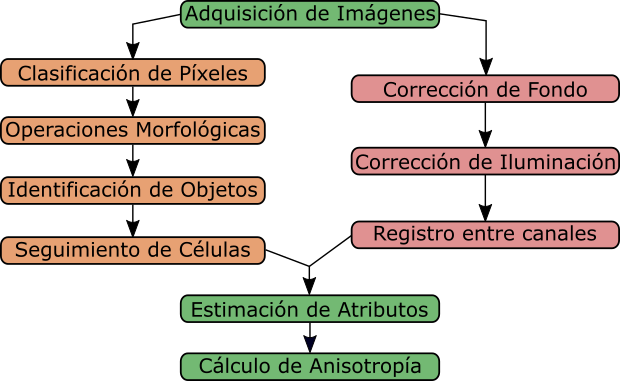
\includegraphics[width=0.7\textwidth]{img/cap_2/analysis_pipeline.png}
    \caption{\footnotesize{Esquema del procedimiento de análisis de imágenes utilizado. Luego de la adquisición de imágenes el proceso se divide en dos que pueden ocurrir en paralelo: segmentación y seguimiento de células; y corrección y cuantificación de intensidad. Una vez segmentadas las células y corregidas las imágenes, se pueden estimar diversos atributos de ellas (tamaño, excentricidad, intensidad de fluorescencia, etc) y luego calcular su anisotropía.}}
    \label{fig:analisis_imagenes}
\end{figure}


%%%%%%%%%%%%%%%%%%%%%%%%%%%%%%%%%%
\subsection{Segmentación y Seguimiento de Células}


En primer lugar, para obtener la información buscada en las imágenes debemos segmentarlas. Este paso consiste en clasificar qué píxeles corresponden a objetos y cuáles a fondo. Existen diversas formas de realizar esta clasificación, desde utilizar un valor umbral para clasificar los píxeles, o primero utilizar kernels específicos para resaltar alguna característica en la imagen, hasta algoritmos de aprendizaje automático donde se utilizan grandes librerías de imágenes ya segmentadas para generar un algoritmo que aprenda a distinguir entre cada clase de píxeles.

Para la clasificación de píxeles se utilizó un algoritmo desarrollado en el laboratorio que se encuentra disponible para descargar de \href{https://github.com/maurosilber/cellment/tree/master/cellment}{Cellment} (ver apéndice \ref{repositorio}). Dicho algoritmo analiza los gradientes de intensidad en la imagen para detectar píxeles que con certeza pertenecen al fondo de la imagen (\cref{fig:clasificacion}B y \ref{fig:clasificacion}C). A partir de estos es capaz de reproducir de forma robusta la distribución de intensidad de los píxeles del fondo. Luego, se puede elegir como umbral para clasificar píxeles algún percentilo de dicha distribución (\cref{fig:clasificacion}A). Para la clasificación se utilizó el percentilo 70 de la distribución de intensidad del fondo (\cref{fig:clasificacion}D).

\begin{figure}[htb]
    \centering
    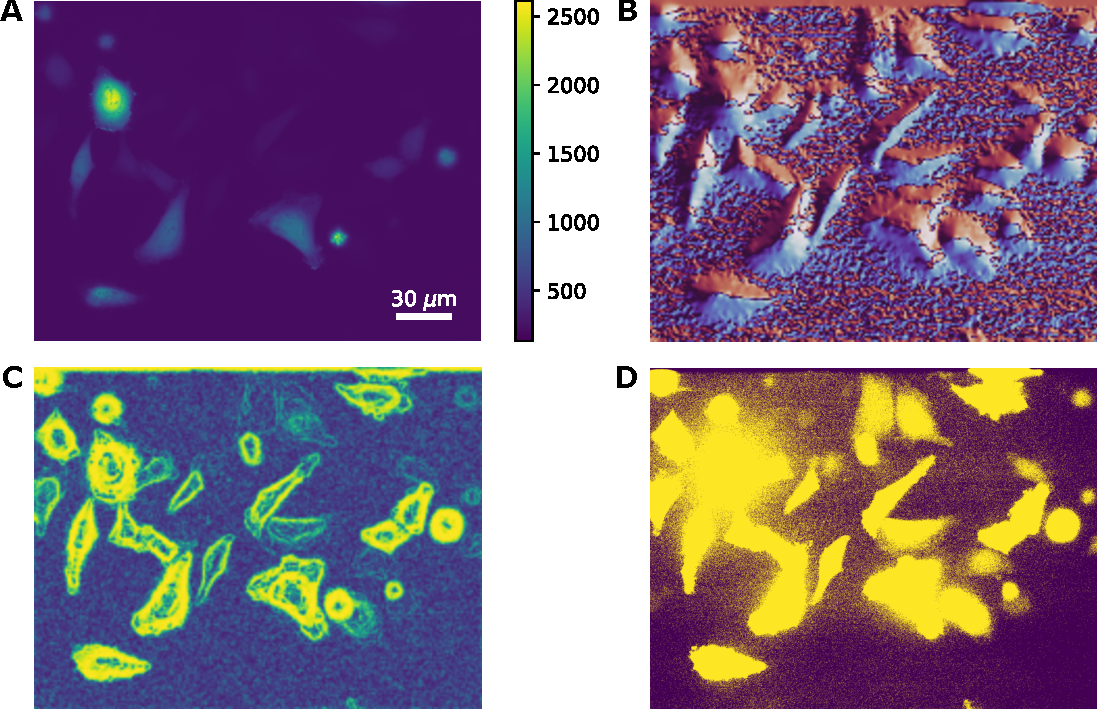
\includegraphics[width=0.9\textwidth]{img/cap_2/clasificacion.pdf}
    \caption{\footnotesize{Análisis de imágenes que lleva a la clasificación de píxeles en fondo y frente. Cabe destacar que aunque las células se vean tenues en la imagen original, es posible distinguirlas en la clasificación. \textbf{A.} Imagen característica de una posición dentro de un pocillo del LabTek de un experimento donde se utilizó staurosporina como estímulo apoptótico. \textbf{B.} Imagen que resulta de estudiar la direccionalidad del gradiente de la imagen cruda suavizada. Este paso es una ayuda visual para interpretar como incrementa la intensidad de fluorescencia desde el borde de la célula al centro debido a su forma. \textbf{C.} Imagen resultante de aplicar el filtro \ening{Silver Mountain Operator} (SMO) a la imagen analizada. Dicho filtro es un paso esencial del análisis utilizado en el algoritmo de Cellment. \textbf{D.} Habiendo hallado la distribución de intensidad del fondo, se utilizó el valor del percentilo 70 para clasificar píxeles en fondo y frente. Notar el patrón en sal y pimienta resultante en la imagen que será corregido en los próximos pasos.}}
    \label{fig:clasificacion}
\end{figure}

Una vez seleccionados los píxeles correspondientes a objetos en la imagen, es necesario eliminar artefactos de la clasificación. Estos se dan principalmente cuando píxeles del fondo toman valores elevados debido a ruido en la medición, formando patrones llamados sal y pimienta, o en los bordes de los objetos ya que las intensidades son bajas y comparables al fondo (\cref{fig:clasificacion}D). Para corregir patrones en sal y pimienta se pueden utilizar métodos que remueven objetos o agujeros pequeños, ya que estos son considerablemente menores que el tamaño típico de nuestro objeto de interés. Por otro lado, hay operaciones morfológicas que consisten en cambiar la clase de un píxel según si en su vecindad hay un píxel correspondiente a fondo (erosión) o frente (dilación). Estas operaciones se pueden aplicar sucesivamente para suavizar bordes, conectar estructuras e incluso eliminar el patrón en sal y pimienta. Notar que el orden en que se aplica la erosión y dilación no es indistinto y se denominan apertura, erosión seguido de dilación, y clausura, el orden inverso. Particularmente, se aplicó una clausura definiéndose como vecindad un disco de radio 10 píxeles (\cref{fig:seguimiento}A y B).

Luego de separar los píxeles correspondientes al frente y fondo, debemos separar el frente en cada uno de los objetos que lo componen, en este caso, células. En raras ocasiones, las células se encuentran suficientemente alejadas unas de otras como para ser identificadas como objetos separados, mientras que en la mayoría de los casos debemos separarlas por otros métodos. Si tenemos en cuenta que, dada la morfología celular, el centro de las células es más intenso que los bordes, se pueden utilizar algoritmos como \ening{watershed} para separarlas. Este algoritmo toma como entrada semillas que marcan las posiciones en donde hay células y luego utiliza la topografía formada por la intensidad de la imagen para separarlas entre sí. Como punto de partida, se utilizaron los máximos locales de intensidad (\cref{fig:seguimiento}C y D).

\begin{figure}[htb]
    \centering
    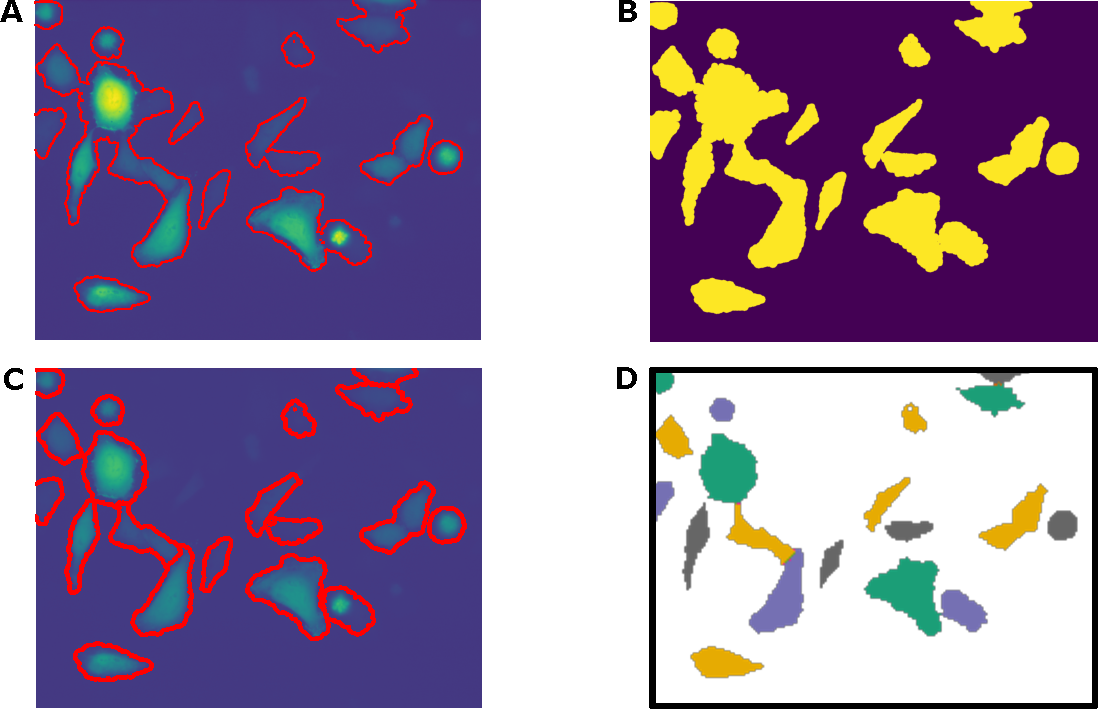
\includegraphics[width=0.9\textwidth]{img/cap_2/seguimiento.pdf}
    \caption{\footnotesize{Análisis de imágenes que permitió reconocer objetos (células) y seguirlos a lo largo de la serie temporal. \textbf{A.} Imagen de ejemplo analizada con el contorno que resulta de aplicar operaciones morfológicas sobre la imagen de clasificación de píxeles. \textbf{B.} A la clasificación presentada en la \cref{fig:clasificacion}D se le aplico una operación morfológica de clausura definiendo como vecindad un disco de radio 10 píxeles. \textbf{C.} Imagen de ejemplo analizada con el contorno de las células reconocidas por el algoritmo de seguimiento. \textbf{D.} Imagen que resulta de separar en las distintas células, luego del análisis de seguimiento, los objetos hallados en el frente de la imagen presentada en \textbf{B}.}}
    \label{fig:seguimiento}
\end{figure}

Habiendo identificado a las células como objetos distintos en las sucesivas imágenes, y sabiendo que estas pueden trasladarse a lo largo del experimento, será necesario seguirlas a lo largo de la serie temporal. Dado que el traslado de las células en estudio es chico en relación a su área en esta escala de tiempo, esto se logró comparando el área superpuesta entre objetos en imágenes subsiguientes. Puede darse la situación en que la cantidad de objetos detectados sea distinta entre imágenes. En algunos casos, esto puede deberse a que hubieron defectos en segmentación y separación de células contiguas. Esta información es utilizada para separar células que no fueron adecuadamente separadas en los pasos previos. En el caso de experimentos de apoptosis, esto es fácil de identificar cuando células contiguas se desprenden del vidrio en momentos distintos ya que cambian su forma y se separan una de otra, siendo fácilmente separables. Esta información puede utilizarse para separar las células en imágenes previas (\cref{fig:seguimiento}D y \cref{fig:track_many}).

\begin{figure}
    \centering
    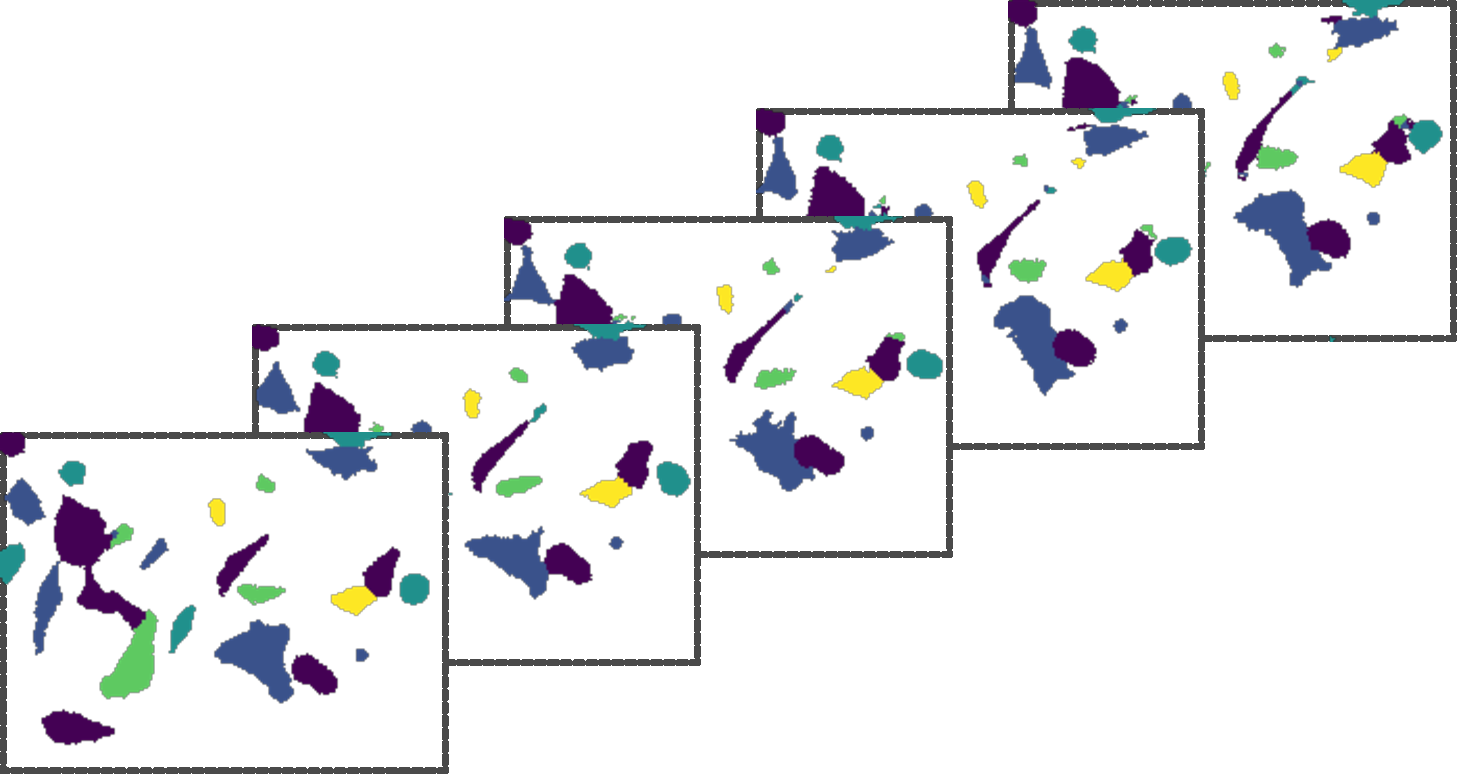
\includegraphics[width=0.7\textwidth]{img/cap_2/tracking_many.pdf}
    \caption{\footnotesize{Secuencia de imágenes de ejemplo para mostrar el algoritmo de seguimiento de células. Se muestran una de cada 5 imágenes correspondientes a la imagen de muestra utilizada previamente. Cada color corresponde a una célula distinta que fue seguida a lo largo de la secuencia.}}
    \label{fig:track_many}
\end{figure}


%%%%%%%%%%%%%%%%%%%%%%%%%%%%%%%%%
\subsection{Estimación de Anisotropía}
\label{sec:matmet:CalculoAnisotropia}


Una vez segmentadas las células y habiendo completado el seguimiento de ellas a lo largo de la serie temporal, debemos estimar su intensidad de fluorescencia en cada imagen. Para ello será necesario aplicar primero diversas correcciones a las imágenes. Por ejemplo, corregir inhomogeneidades en la iluminación, el fondo y posibles desplazamientos entre los canales adquiridos (\cref{fig:analisis_imagenes}). Además, por tratarse de anisotropía de fluorescencia, será necesario corregir el factor G, es decir, las diferencias en ganancia y depolarizaciones que pueden haber en la adquisición de las distintas polarizaciones.

El primer paso fue corregir el fondo de las imágenes. Para ello, se aprovechó que conocíamos con bastante certeza los píxeles correspondientes al fondo y sus posiciones. Esto ayudó a generar una imagen que surgía de interpolar una superficie suave que pase por los píxeles oscuros detectados (\cref{fig:correcciones}A). A nuestra imagen de interés le debemos restar la superficie interpolada. Luego discutiremos los efectos en el cálculo de anisotropía que surgen de errores en la estimación de fondo.

\begin{figure}[htb]
    \centering
    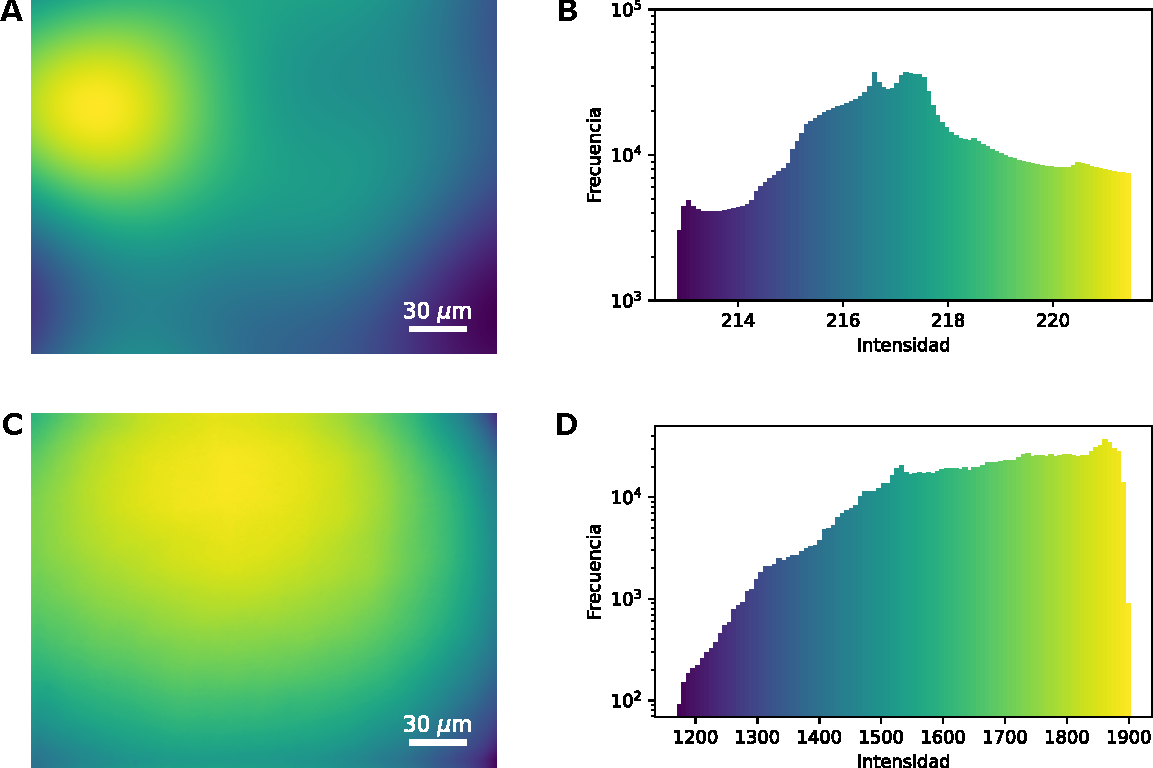
\includegraphics[width=0.9\textwidth]{img/cap_2/correcciones.pdf}
    \caption{\footnotesize{Imágenes de fondo e iluminación utilizadas para corregir las imágenes obtenidas. \textbf{A.} Imagen del fondo estimado para el ejemplo analizado. Las inhomogeneidades corresponden al brillo  fuera de foco de las células. Cabe destacar que las diferencias de intensidades son del orden de la decena. \textbf{B.} Histograma de intensidades correspondientes al fondo estimado. Notar que los valores se encuentran alrededor de 200 que corresponden al fondo de la cámara. \textbf{C.} Imagen correspondiente a la normalización utilizada. Esta imagen surge de calcular la mediana píxel a píxel de varias imágenes de fluoresceína diluida. \textbf{D.} Histograma de intensidades correspondientes a la imagen de normalización obtenida. Notar que la población de píxeles poco iluminados es considerablemente menor que los más iluminados.}}
    \label{fig:correcciones}
\end{figure}

A continuación, se corrigieron las inhomogeneidades en la iluminación. Para ello, se adquirieron diez imágenes de fluoresceína diluida en cada polarización utilizando el mismo armado experimental. Se generó una única imagen que consistió en la mediana para cada píxel de las distintas imágenes (\cref{fig:correcciones}C). Ésta imagen fue utilizada para realizar una división píxel a píxel de todas las imágenes adquiridas. Como se mencionó previamente, la fluoresceína diluida tiene un valor nulo de anisotropía y, por lo tanto, también sirve como corrección de factor G. En la figura \ref{fig:correcteds} puede apreciarse el resultado de aplicar las sucesivas correcciones.

\begin{figure}[htb]
    \centering
    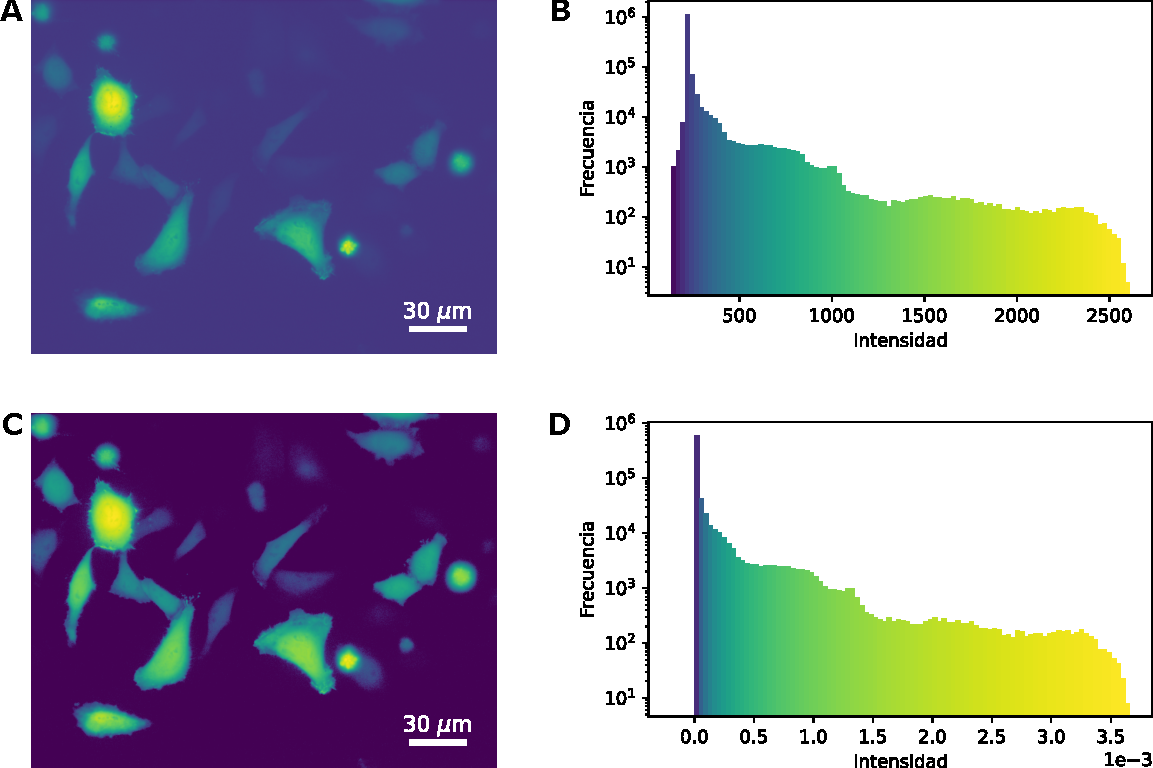
\includegraphics[width=0.9\textwidth]{img/cap_2/correcteds.pdf}
    \caption{\footnotesize{Imágenes original y corregida con sus respectivos histogramas de intensidad. \textbf{A.} Imagen de ejemplo analizada. \textbf{B.} Histograma de intensidades obtenidos de la imagen que será analizada. Notar que la cámara de 12 bits tiene un rango dinámico de hasta 4096 y se decidió no usar la totalidad de éste para que no saturen las imágenes subsiguientes. \textbf{C.} Imagen corregida que resulta de restarle el fondo y normalizar a la imagen original. \textbf{D.} Histograma correspondiente a la imagen corregida. Se puede apreciar que los valores de intensidad corresponden a las distintas células presentes en la imagen.}}
    \label{fig:correcteds}
\end{figure}

Corregir adecuadamente la inhomogeneidad en la iluminación, el fondo y factor G es esencial para una correcta estimación de la intensidad de fluorescencia. Por medio de un código interactivo (\href{https://github.com/acorbat/anisotropy_errors/tree/master/anisotropy_errors}{anisotropy\textunderscore errors}, ver apéndice \ref{repositorio}) se analizó la propagación de cometer errores en la estimación de intensidad paralela o perpendicular. Es trivial notar que un error sistemático trasladará y reescalará la curva de anisotropía. Es decir, la forma se mantendrá pero la anisotropía del dímero y monómero serán distintos a lo esperado (ver \cref{fig:error_bkg}). Por otro lado, dependiendo de la magnitud de este error, podría ocurrir que la anisotropía del monómero sea menor que la del dímero, produciendo una inversión de la curva. Por último, debemos destacar que si el error varía a lo largo del tiempo, esto puede cambiar la forma de la curva y llevar a mayor confusión y dificultad a la hora de corregirlo.

\begin{figure}[htb]
    \centering
    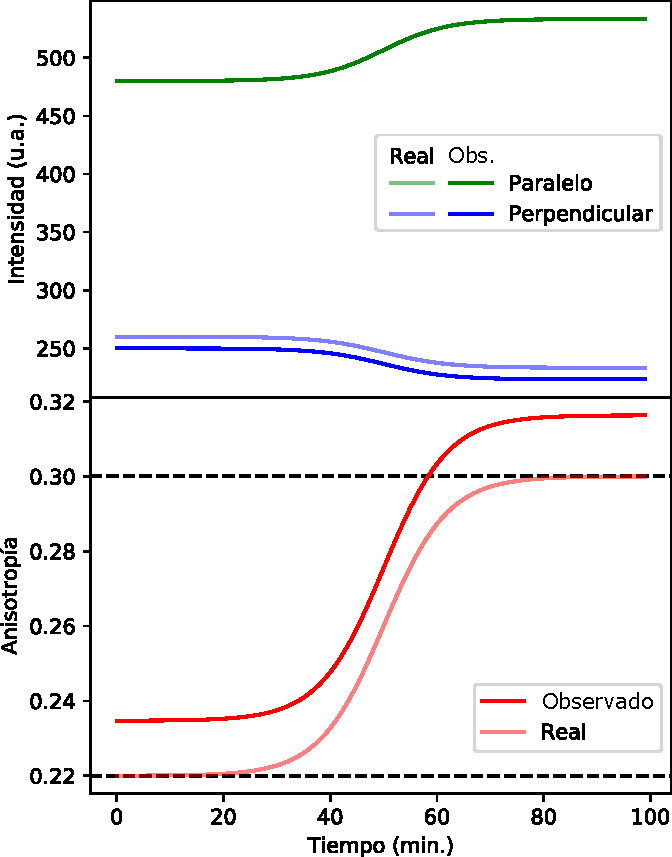
\includegraphics[width=0.5\textwidth]{img/cap_2/error_bkg.pdf}
    \caption{\footnotesize{Simulación de curvas de intensidad paralela y perpendicular donde se cometió un error de solo 10 unidades en la estimación del fondo de la imagen perpendicular, que corresponde a menos del 5\%. Dicho error se traduce en un corrimiento de la curva de anisotropía de 0.02 que representa alrededor de un 10\%.}}
    \label{fig:error_bkg}
\end{figure}

Luego, debemos corregir posibles desplazamientos entre las imágenes de los distintos canales. Aunque este efecto suele ser pequeño cuando se utilizan distintos filtros de emisión, es mucho más pronunciado al cambiar de polarizador. Esto se debe principalmente a que los polarizadores utilizados son gruesos (7~mm) ya que el grosor se asocia a su calidad. Si consideramos al polarizador como dos cambios de medio paralelos, podemos realizar un análisis de trayectoria de rayos para entender que si el haz incide en algún ángulo no perpendicular, el polarizador trasladará el haz una distancia que dependerá de su grosor, sin afectar su direccionalidad.

\begin{figure}[b!]
    \centering
    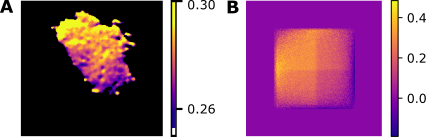
\includegraphics[width=0.6\textwidth]{img/cap_2/shifts.png}
    \caption{\footnotesize{Imágenes de anisotropía calculadas a partir de imágenes de intensidad que están desplazadas una respecto de la otra. \textbf{A.} Imagen correspondiente a una célula observada experimentalmente. Puede apreciarse que en la región superior los valores de anisotropía calculados son más altos que en la sección inferior. \textbf{B.} Imagen de anisotropía generada a partir de una célula con forma piramidal simulada utilizando anisotropy\textunderscore errors.}}
    \label{fig:shifts}
\end{figure}

El patrón generado en la imagen de anisotropía por este tipo de errores de registro entre canales es fácilmente identificable y se aprecia como sombras topográficas (ver  \cref{fig:shifts}). Consideremos un objeto con un gradiente de intensidad, como suele suceder en el citoplasma de algunas células. Al estar desplazadas las imágenes, siempre se restarán valores desfasados del gradiente de intensidad. Esto resultará en que los valores de anisotropía estarán corridos hacía valores mayores o menores dependiendo de la dirección del gradiente respecto a la dirección del desplazamiento, generando una imagen de aspecto sombreada. Esto se exacerba aún más en los píxeles del borde del objeto, donde alguna de las intensidades será casi nula por corresponder al fondo, resultando en valores extremos de anisotropía.

Mediante simulaciones de imágenes de intensidades paralela y perpendicular (ver \href{https://github.com/acorbat/anisotropy_errors/tree/master/anisotropy_errors}{anisotropy\textunderscore errors} y \cref{fig:shifts}) se estudió la forma más robusta de estimar la anisotropía de cada objeto. A grandes rasgos y considerando que el cálculo de anisotropía es no lineal, es posible calcular la imagen de anisotropía y promediar los valores obtenidos o promediar en las imágenes de intensidades y calcular la anisotropía. Cabe destacar que si quisiéramos calcular la imagen de anisotropía, debemos ser capaces de corregir ambas imágenes de intensidad lo mejor posible. En el caso de corregir desplazamientos entre imágenes, puede ser necesario hacer una traslación subpíxel, es decir, una distancia menor al tamaño de un píxel. Para lograr esto último sería necesario interpolar entre los píxeles adquiridos de la imagen, proceso que suele incrementar el ruido.

\begin{figure}[t!]
    \centering
    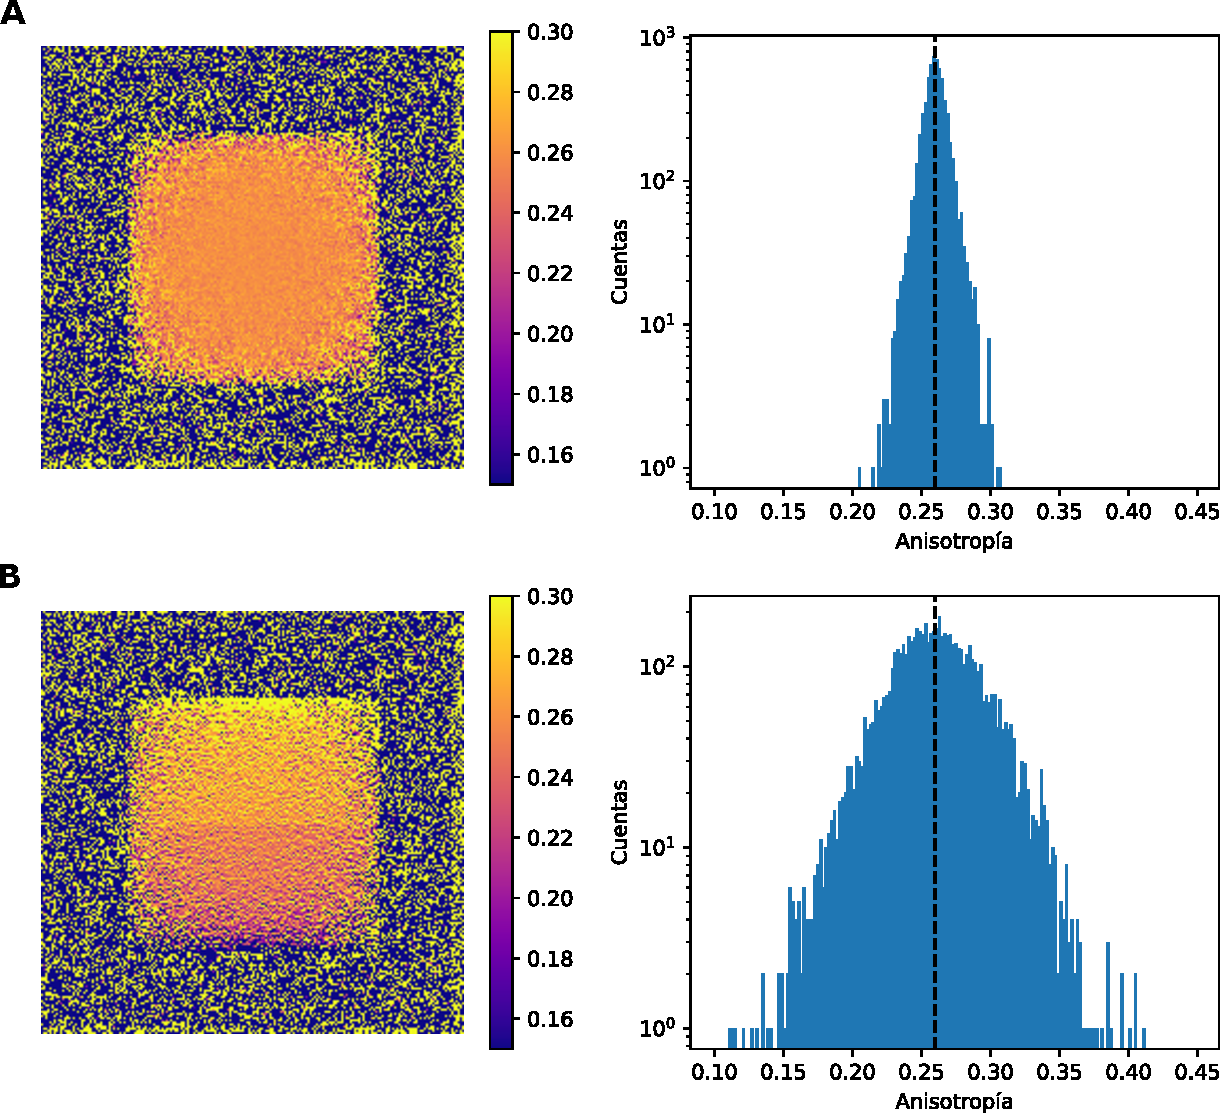
\includegraphics[width=0.75\textwidth]{img/cap_2/anisotropy_variances.pdf}
    \caption{\footnotesize{Si simularon células de forma piramidal con los biosensores dentro tomados de distribuciones al azar. El ensamble de biosensores se simuló de tal forma que su anisotropía sea 0.26. A la izquierda se ven las imágenes de anisotropía de las célula adquiridas y corregidas perfectamente (\textbf{A}) o con un shift de un píxel en el eje vertical (\textbf{B}). A la derecha se grafican los histogramas de anisotropía de los píxeles de la célula, ignorando el borde de esta ya que es muy ruidoso debido a la baja intensidad. Se puede apreciar que este leve error en la corrección del corrimiento no solo generó una imagen fácilmente distinguible, sino que también esto hace que la varianza aumente considerablemente. Notar que con un pequeño corrimiento de un píxel la media no varía de forma apreciable, pero este efecto será mayor para corrimientos más grandes. Por otro lado, si el corrimiento es menor a un píxel, es necesario interpolar los valores entre píxeles y esto puede exacerbar el ruido de cada píxel.}}
    \label{fig:anisotropy_variance}
\end{figure}

Se comprobó que errores de registro aumentan la variabilidad de la anisotropía de la célula adquirida, por lo que se consideró barrer en los valores de desplazamiento y minimizar dicha varianza (ver \cref{fig:anisotropy_variance}). Más allá del costo computacional elevado que tenía este procedimiento, se verificó que estimar la suma de intensidades y luego calcular la anisotropía no solo era más eficiente, sino también más robusto. Esto se debía principalmente a que al promediar las intensidades cualquier error de registro remanente era compensado por otras regiones del objeto. Además, al erosionar las células era fácil descartar los píxeles del borde correspondientes a los menos intensos. Por último, calcular la sumatoria de intensidades, equivalente al promedio ya que la anisotropía se normaliza, antes del cálculo de anisotropía es estadísticamente favorable ya que el ruido de cada píxel no se propaga a través del cálculo no lineal.


%%%%%%%%%%%%%%%%%%%%%%%%%%%%%%
\section{Modelado de la Cinética Enzimática}
\label{sec:CineticaEnzimatica}


Las enzimas son catalizadores, en general proteínas, que colaboran en la conversión de sustratos en producto, manteniéndose inalteradas una vez terminada la reacción. Entre sus características más importantes encontramos su elevado poder catalítico, su especificidad y la posibilidad de regularlas. Estas son especialmente eficientes para acelerar reacciones biológicas, aumentando hasta 10 millones de veces la velocidad de reacción. Típicamente se encuentran reguladas por una complicada red de lazos de retroalimentación, tanto positivos como negativos, permitiendo un control preciso sobre la tasa de reacción \citep{Keener2009}.

Las caspasas en estudio son enzimas, en particular, proteasas. Realicemos el experimento mental de modelar un biosensor de caspasas, o cualquier proteasa, como el introducido en el trabajo de \cite{Stegemann2015}. Esto nos servirá para comprender su funcionamiento y entender las razones detrás de cada paso del análisis de datos. Estos biosensores son sintetizados por la célula en su estado dimérico y luego procesados por la caspasa en cuestión una vez activa. Esto es análogo a un sustrato, biosensor dimérico, que es procesado por una enzima, caspasa, para dar lugar de forma irreversible a un producto, biosensor monomérico.

Un modelo para describir esta cinética fue propuesto por Michaelis y Menten. En el esquema de la reacción, la enzima ($E$) convierte al sustrato ($S$) en producto ($P$) en un proceso de dos pasos. En el primer paso, se unen la enzima y el sustrato formando un complejo enzima-sustrato ($C$); para luego dar lugar a la formación del producto y la liberación de la enzima. Esta reacción puede representarse como

\begin{center}
\ce{S + E <=>[$k_+$][$k_-$] C ->[$k_c$] P + E.}
\end{center}

\noindent Aunque en general el producto puede volver a unirse a la enzima, y estas aceleran las reacciones en ambos sentidos, en nuestro caso particular, el biosensor una vez clivado no vuelve a su estado dimérico.

El siguiente paso consiste en aplicar ley de acción de masas para describir el cambio en la concentración de cada una de las especies a partir las constantes cinéticas de cada reacción. Comencemos por considerar una reacción simple en la que el sustrato $S$ y la enzima $E$ colisionan para formar $C$, es decir,

\begin{center}
\ce{S + E ->[$k_+$] C,}
\end{center}

\noindent donde $k_+$ se denomina la constante de reacción. Ésta surge de considerar que las colisiones de las moléculas en el sistema en equilibrio térmico se dan de forma completamente aleatoria. Esta constante depende a su vez de la relación entre los tamaños de las especies involucradas, su geometría y otros parámetros que pueden reducirse a la probabilidad de encuentro y reacción exitosa \citep{Gillespie1977}.

Asumiendo que la concentración de las especies en estudio pueden ser descriptas mediante funciones continuas, y que cada una de sus reacciones químicas pueden representarse como procesos continuos, es posible construir una serie de ecuaciones diferenciales acopladas que describan la dinámica. En este caso particular, la variación de la concentración del complejo ($C$) descripta por \cite{Gillespie1977} es

\begin{equation}
    \frac{dC}{dt} = k[S][E],
\end{equation}

\noindent donde $[S]$ y $[E]$ se refieren a las concentraciones de sustrato y enzima respectivamente. Al igual que la ley de Ohm o la ley de Newton para enfriamiento, esta tiene cierto rango de validez. En primer lugar, si se trabaja a concentraciones altas, duplicar la concentración no implica que necesariamente se duplique la tasa de formación de producto. En el otro extremo, si se utilizan concentraciones muy bajas, puede que representar la concentración como una variable continua no sea la mejor opción \citep{Keener2009}.

Analicemos las ecuaciones diferenciales que surgen al aplicar ley de acción de masas al sistema completo

\begin{align}
    \frac{ds}{dt} =& k_- c - k_+ se \label{eq:cin_sens}\\
    \frac{de}{dt} =& (k_- + k_c) c - k_+ se\\
    \frac{dc}{dt} =& k_+ se - (k_- + k_c) c\\
    \frac{dp}{dt} =& k_c c, \label{eq:cin_prod}\\
\end{align}

\noindent donde se uso que $[E]=e$, $[S]=s$, $[C]=c$ y $[P]=p$. Podemos apreciar que $\frac{de}{dt} + \frac{dc}{dt} = 0$, que corresponde a la existencia de una cantidad conservada, en este caso la enzima. Esto se condice con lo explicado previamente ya que la enzima acelera la reacción, pero se mantiene inalterada una vez culminada. De aquí que $e+c=e_0$ donde $e_0$ es la cantidad de enzima disponible. Por otro lado, también se aprecia que $\frac{ds}{dt} + \frac{dc}{dt} + \frac{dp}{dt} = 0$, que, dado que no hay síntesis de sustrato ni degradación de producto incluidas hasta ahora, se conserva la cantidad de sustrato más producto en todos sus estados.

\begin{figure}[b!]
    \centering
    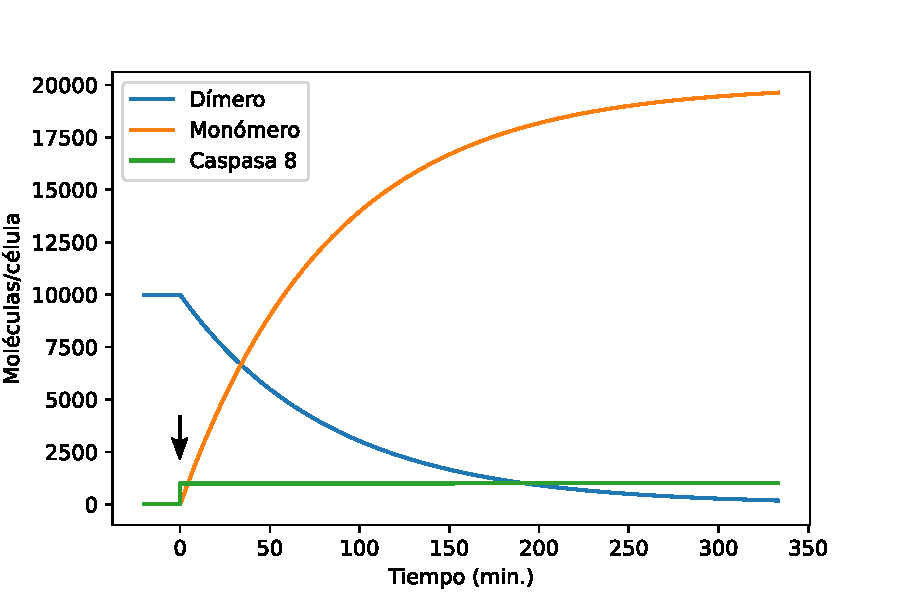
\includegraphics[width=0.6\textwidth]{img/cap_2/ejemplo_enzima.pdf}
    \caption{\footnotesize{Simulación a modo de ejemplo donde la caspasa 8 procede a clivar su biosensor correspondiente. Se comenzó con una concentración inicial de 10000 moléculas de biosensor y a tiempo cero se agregan 1000 moléculas por célula de la caspasa 8. Notar que a tiempos largos, la cantidad de moléculas por celula de biosensor clivado es el doble que la de biosensors dimérico al principio debido a que pasó a estado monomérico. Las constantes cinéticas seleccionadas fueron similares a las encontradas en modelos publicados.}}
    \label{fig:ejemplo_enzima}
\end{figure}

A modo de ejemplo, creemos un modelo en PySB \citep{Lopez2013} en donde vamos a definir las reacciones correspondientes al clivaje de un biosensor dimérico por parte de la caspasa 8. Utilizaremos como constantes cinéticas valores típicos hallados en la bibliografía, a saber, $k_+ = 10^{-7}$, $k_- = 10^{-3}$ y $k_c = 1$. En cuanto a concentraciones iniciales, utilizaremos 1000 moléculas por célula de caspasa 8 y 10000 moléculas de biosensor en estado dimérico. Podemos apreciar que una vez clivado todo el sensor, tendremos 20000 moléculas por célula de biosensor en estado monomérico (ver \cref{fig:ejemplo_enzima}).

Notemos que el biosensor utilizado es irreversible, por lo que no mide directamente la actividad de la caspasa, sino su integral. Utilizando la ecuación \ref{eq:cin_prod} que relaciona la velocidad de formación de producto, o sensor clivado en este caso, con la concentración de complejo, podemos interpretarla como la cantidad de caspasa que se encuentra clivando sensor en cada instante, es decir, ofrece una lectura sobre la actividad caspasa.


%%%%%%%%%%%%%%%%%%%%%%%
\section{Estimación del Observable Biológico}
\label{sec:Observable}


A continuación, debemos traducir los valores de anisotropía hallados para cada célula en una propiedad que refiera a la caspasa, o enzima, en estudio. Supongamos entonces una población de biosensores con una concentración ($[C]$) que se encuentra una parte en estado dimérico ($[D]$) y otra en estado monomérico ($[M]$). Si tenemos en cuenta que los distintos fluoróforos poseen propiedades fotofísicas diferentes, como sus espectros de absorción y emisión, su rendimiento cuántico, el estado madurativo de los fluoróforos que lo componen, entre otras, entonces sus brillos por molécula detectados serán diferentes. Esto quiere decir que las intensidades de cada subpoblación de fluoróforos será

\begin{align}
    I_M &= (b_{M_1} + b_{M_2}) M\\
    I_D &= (b_{M_1} + b_{M_2} + \delta b) D,
\end{align}

\noindent donde se asumió que la concentración de cada tipo de fluoróforo en estado monomérico es igual ya que los biosensores se sintetizan como dímeros y luego son clivados. Los brillos de cada fluoróforo son $b_{M_1}$ y $b_{M_2}$, mientras que en el caso del dímero, a estos brillos se les suma $\delta b$ ya que debido a la transferencia de energía entre ellos, el brillo detectado dependerá de qué fluoróforo emita con mayor intensidad.

\begin{figure}[htb]
    \centering
    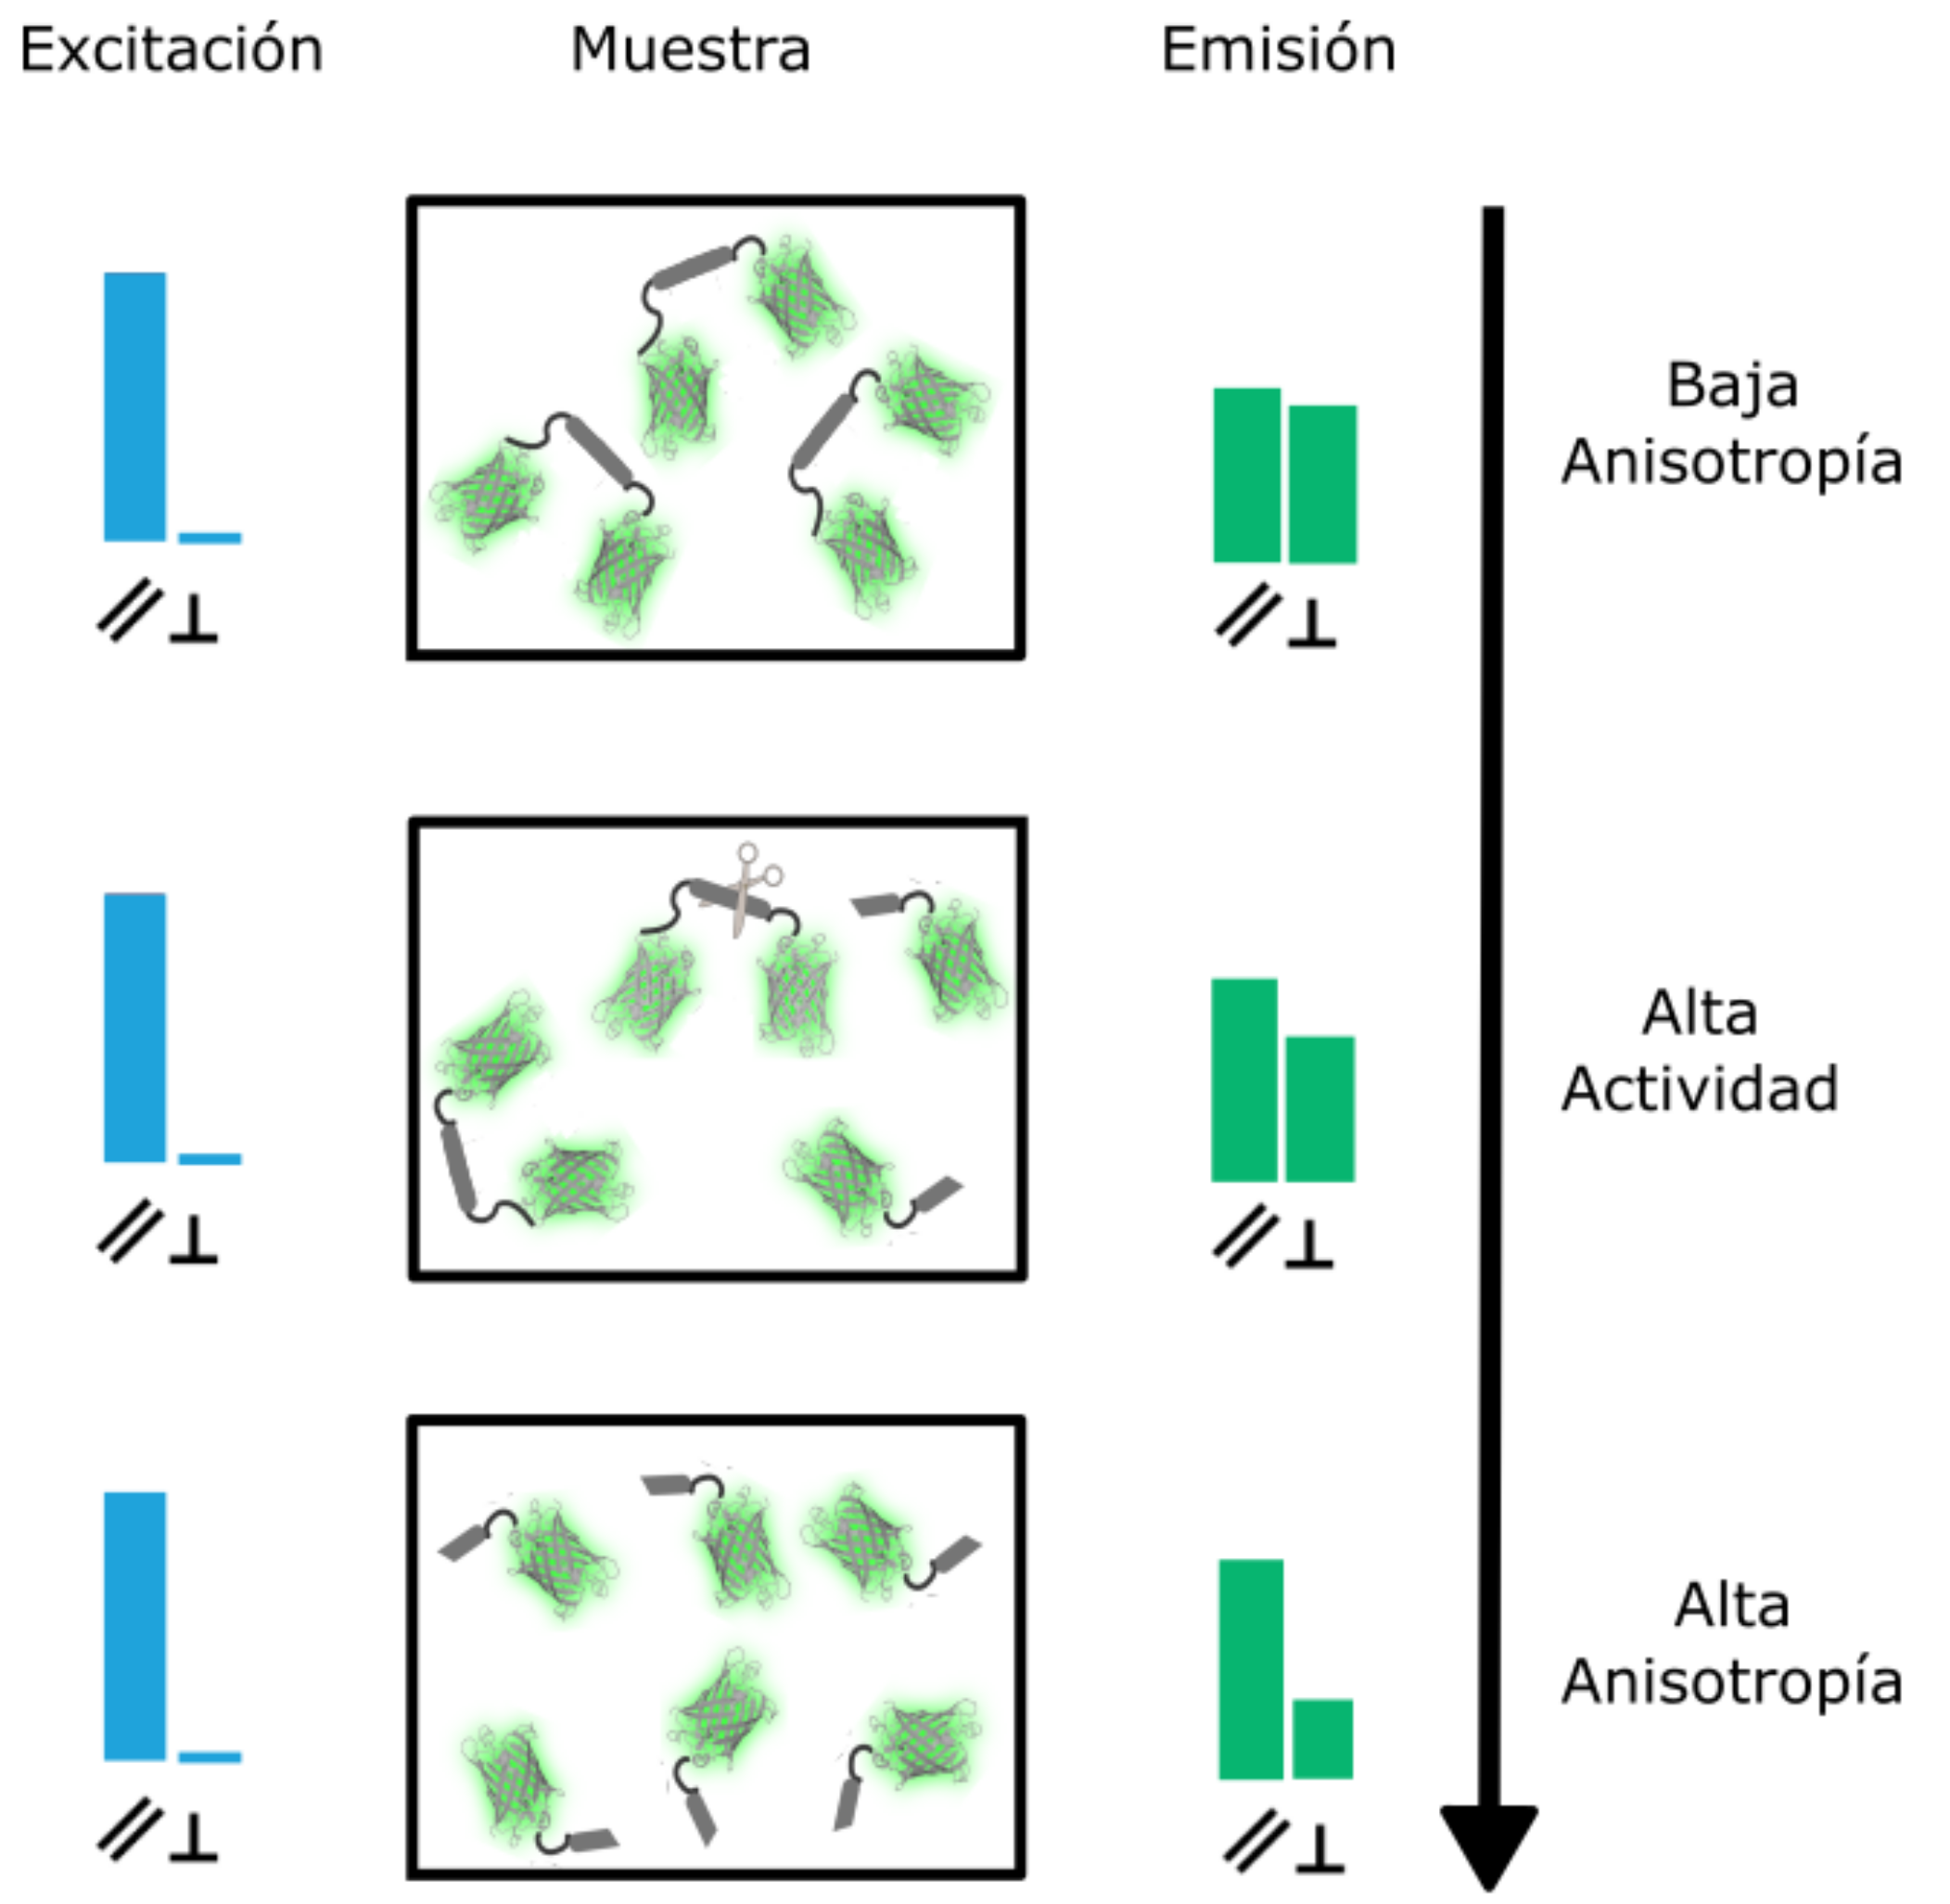
\includegraphics[width=0.6\textwidth]{img/cap_2/anisotropy_sensors.png}
    \caption{\footnotesize{Los biosensores son sintetizados en forma dimérica por las células y en este estado tienen una anisotropía de polarización baja debido a FRET entre fluoróforos. Una vez clivados, estos biosensores no pueden volver al estado previo y sirven como reporteros de la actividad integral de las caspasas. Al clivarse todo el ensamble de biosensores, se interrumpe el FRET entre fluoróforos y se alcanza un nivel de anisotropía de polarización más elevado. Adaptado de \cite{Corbat2018}.}}
    \label{fig:anisotropia_biosensor}
\end{figure}

Considerando que la anisotropía del conjunto de biosensores nos refiere al estado de dicha población a través del promedio pesado de sus intensidades (ver \cref{fig:anisotropia_biosensor}), es decir, 

\begin{equation}
r = \frac{\sum_i I_i r_i}{\sum_i I_i}, \label{eq:anisotropiaInt}
\end{equation}

\noindent donde $I_i$ corresponde a la intensidad del biosensor en un estado y $r_i$ su anisotropía. Suponiendo además que la concentración de biosensores se mantiene constante, 

\begin{equation}
    [C] = [M] + 2[D],
    \label{eq:C_cte}
\end{equation}

\noindent podemos despejar $m = [M]/[C]$, la fracción de biosensores en estado monomérico en función de las anisotropías

\begin{equation}
	m = \frac{b (r - r_D)}{r_M - r + b (r - r_D)},
	\label{eq:m_from_r}
\end{equation}

\noindent donde $r_D$ y $r_M$ corresponden a las anisotropías del dímero y monómero respectivamente; y donde $b=B_D/B_M = (b_{M_1} + b_{M_2} + \delta b) / (b_{M_1} + b_{M_2})$ es la relación entre brillos. De esta forma, podemos traducir anisotropía en la fracción de biosensor en estado monomérico y viceversa, pasando por valores esperados de intensidad de fluorescencia en cada polarización (ver \cref{fig:mono_to_ani}).

\begin{figure}[htb]
    \centering
    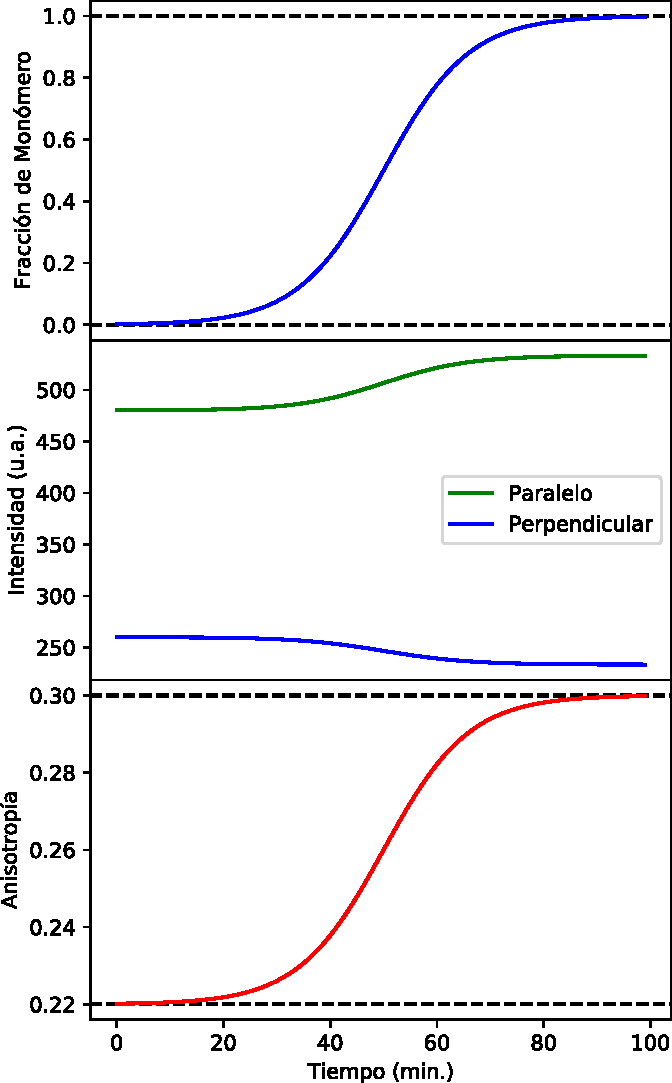
\includegraphics[width=0.5\textwidth]{img/cap_2/mono_to_ani.pdf}
    \caption{\footnotesize{Se generó una curva ejemplo de fracción de biosensor en estado monomérico en función del tiempo y se estimaron sus intensidades en los canales paralelo y perpendicular a la excitación. A continuación, es posible traducir la curva de fracción de monómero, así como las de intensidades, en la curva correspondiente de anisotropía en función del tiempo. Para todo ello es necesario conocer los valores de anisotropía del dímero y monómero, así como $\Delta b$.}}
    \label{fig:mono_to_ani}
\end{figure}

Teniendo en cuenta que el biosensor es irreversible, este solo puede medir la actividad integral de la enzima bajo estudio (\cref{fig:anisotropia_biosensor}). Por esta razón, uno debe calcular su derivada para obtener la actividad enzimática instante a instante (como se menciona al final de la sección \ref{sec:CineticaEnzimatica}), es decir,

\begin{equation}
	\dot{m} = \frac{1 + \Delta b}{r_M - r_D} \frac{\dot{r}}{\left[1 + \Delta b \frac{r - r_D}{r_M - r_D}\right]^2}.
	\label{eq:m_der}
\end{equation}

\noindent donde $1 + \Delta b = (b_{M_1} + b_{M_2} + \delta b) / (b_{M_1} + b_{M_2})$ es la relación entre los brillos del dímero sobre los del monómero. Cabe destacar que dichas propiedades no solo dependen del fluoróforo utilizado sino también del sistema de detección utilizado. Notar que si el brillo detectado de ambos monómeros es igual al del dímero, $\Delta b = 0$, entonces la derivada de la fracción de monómero es proporcional a la derivada de anisotropía (ver \cref{fig:sweep_b}). 

Consideremos el error que se genera al no utilizar el parámetro $\Delta b$. Analicemos brevemente la ecuación \ref{eq:m_der} que nos dice que el máximo de actividad, dado por el máximo de la derivada del cambio de fracción de monómero depende de la derivada de la curva de anisotropía, dividida por $\left[1 + \Delta b \frac{r - r_D}{r_M - r_D}\right]^2$. Donde el segundo término dentro de la potencia es la curva de anisotropía normalizada por sus valores extremos, anisotropía del dímero y monómero, multiplicada por $\Delta b$. Eso quiere decir que el máximo de actividad estará cerca de donde la curva de anisotropía cambie de valor y que éste se verá afectado por el denominador cuando $\Delta b$ sea distinto de 0. Teniendo esto en cuenta, es de esperarse que utilizar un valor erróneo nos dará un error sistemático de unos pocos minutos ya que el transcurso de tiempo en el que cambia la curva es de ese orden (ver \cref{fig:sweep_b}).

\begin{figure}[htb]
    \centering
    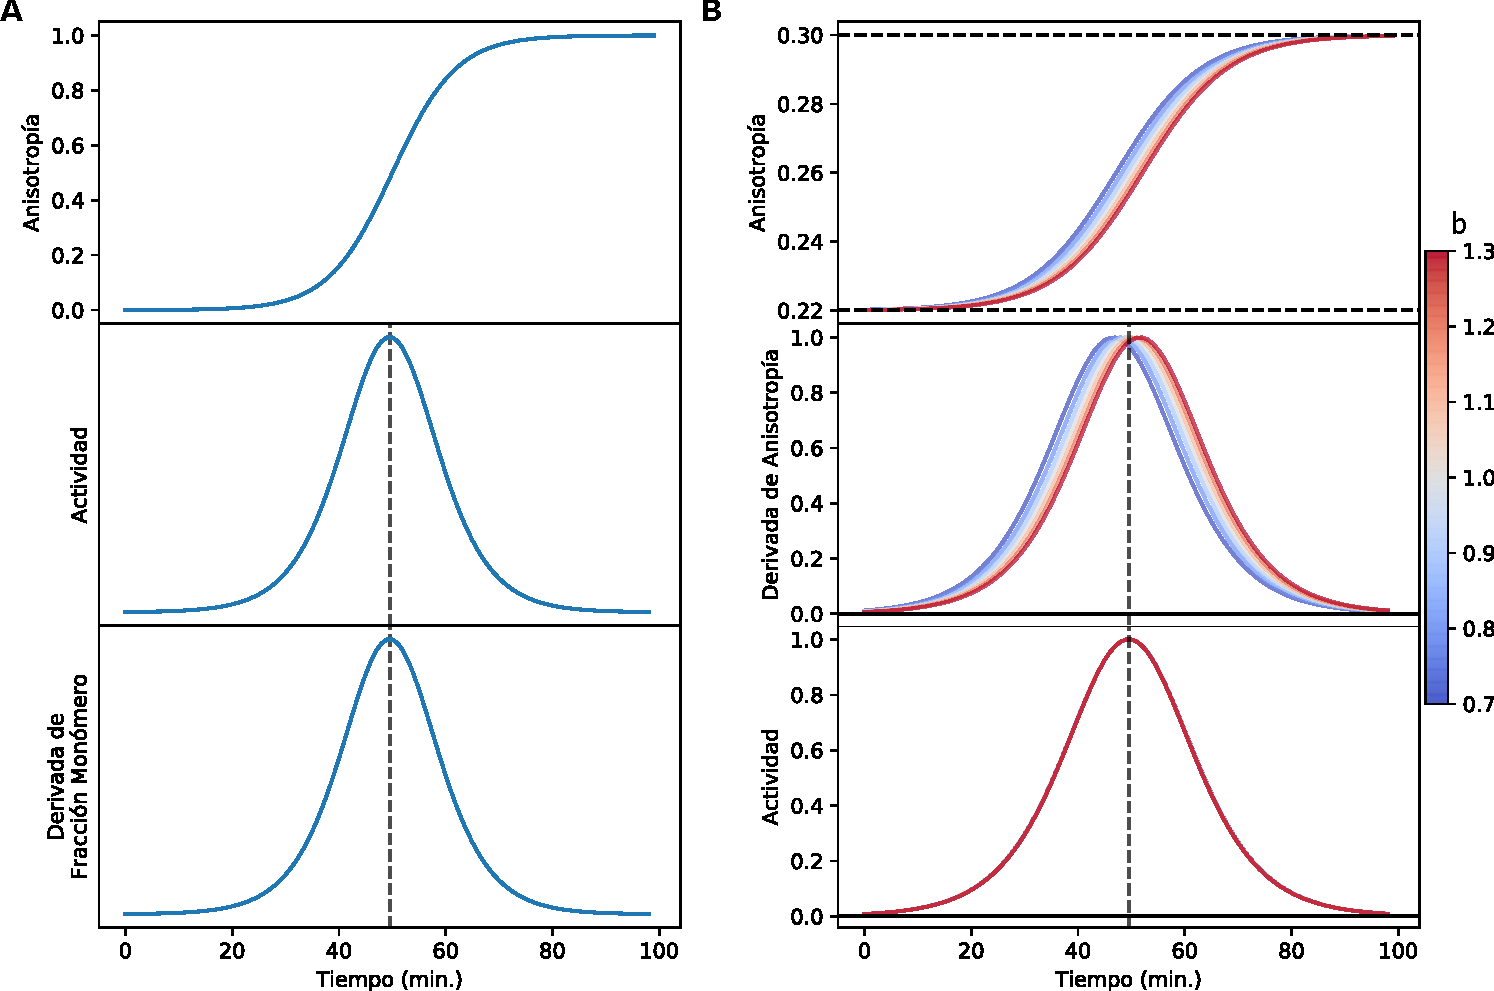
\includegraphics[width=0.9\textwidth]{img/cap_2/sweep_b_mono_ders.pdf}
    \caption{\footnotesize{Sabiendo como traducir la curva de fracción de monómero en anisotropía y viceversa, es posible también calcular la actividad enzimática instante a instante. \textbf{A.} Se simuló una curva de fracción de biosensor en estado monomérico y se muestra la equivalencia entre su derivada y la curva de actividad instante a instante. \textbf{B.} Se simularon curvas de anisotropía a partir de la misma curva de fracción de monómero pero variando el parámetro $\Delta$b entre -0.3 y 0.3, es decir, se varió $b$ entre 0.7 y 1.3. Se puede apreciar como las curvas de anisotropía y sus derivadas se corren dependiendo del valor de b, sin embargo, la curva calculada de actividad es siempre la misma.}}
    \label{fig:sweep_b}
\end{figure}

Conociendo el formalismo teórico detrás del funcionamiento del biosensor utilizado, debemos ser capaces de calcular la actividad enzimática a partir de las curvas de anisotropía obtenidas luego del análisis de imágenes. Para ello, necesitaremos estimar la derivada de las curvas de anisotropía, así como los valores de anisotropía del monómero y dímero. Debido al ruido de alta frecuencia y la necesidad de calcular divisiones donde el denominador suele ser considerablemente menor que el numerador, derivar es una operación computacionalmente mal definida. Por estas razones, se evaluaron distintos métodos para calcular la derivada de las curvas de anisotropía obtenidas a partir del análisis de imágenes. En primer lugar se consideró realizar ajustes con curvas sigmoideas y luego derivarlas, pero no todas las actividades presentaban un perfil sigmoideo por lo que se decidió no proseguir. En segundo lugar, se consideró utilizar diferencias finitas. Aunque dicho algoritmo sopesa adecuadamente los puntos más cercanos para hallar la derivada, tiene problemas cuando hay puntos faltantes. Finalmente, se implementó un filtro savitzky-golay. Dicho filtro hace un ajuste polinomial de bajo grado en una ventana móvil de un número impar de puntos. El valor del polinomio del punto intermedio puede utilizarse para reemplazar el valor de la curva experimental, sirviendo de suavizado, o puede utilizarse para estimar la derivada en dicho punto. La principal desventaja de éste es que al suavizar la curva, el máximo de la derivada puede disminuir aunque no se espera ver un corrimiento pronunciado. Luego se procedió a interpolar con splines de grado 3 para obtener los valores de actividad entre cada punto experimental y tomar el tiempo de máxima actividad (ver \cref{fig:savgol_test}).

\begin{figure}[htb]
    \centering
    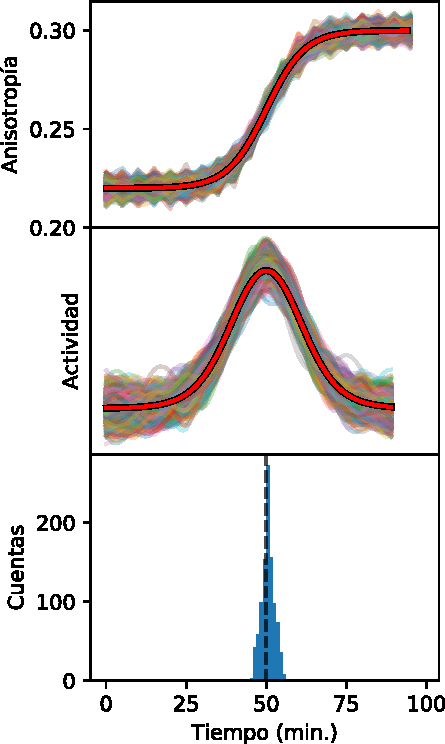
\includegraphics[width=0.4\textwidth]{img/cap_2/savgol_test.pdf}
    \caption{\footnotesize{A partir de una curva de anisotropía simulada se generaron 1000 realizaciones de la misma con ruido experimental añadido y tomando valores cada 5 minutos (superior). Se estimaron las derivadas con el filtro Savitzky-Golay y se procedió a interpolar con splines de grado 3 para obtener los valores de actividad entre cada punto experimental (medio). Finalmente, se tomaron los valores de máximo de actividad devueltos por cada realización y se confeccionó un histograma (inferior). El valor medio recuperado se corresponde con el máximo de actividad estimado de la curva real y el desvío estándar obtenido fue de 1.9 minutos.}}
    \label{fig:savgol_test}
\end{figure}

Finalicemos con un breve análisis de como calcular el denominador de la derivada de la fracción de monómero. Para ello es necesario estimar propiedades fotofísicas de cada biosensor. Por un lado, el valor de $\Delta b$ puede calibrarse a partir de experimentos. Por otro lado, los valores de anisotropía de dímero y monómero se estimaron para cada curva en particular ya que, como se discutió previamente, son susceptibles a variar debido a la propagación de errores. Una estimación típica de la curva de actividad a partir de la anisotropía se halla en la \cref{fig:derivacion_tipica}.

\begin{figure}[htb]
    \centering
    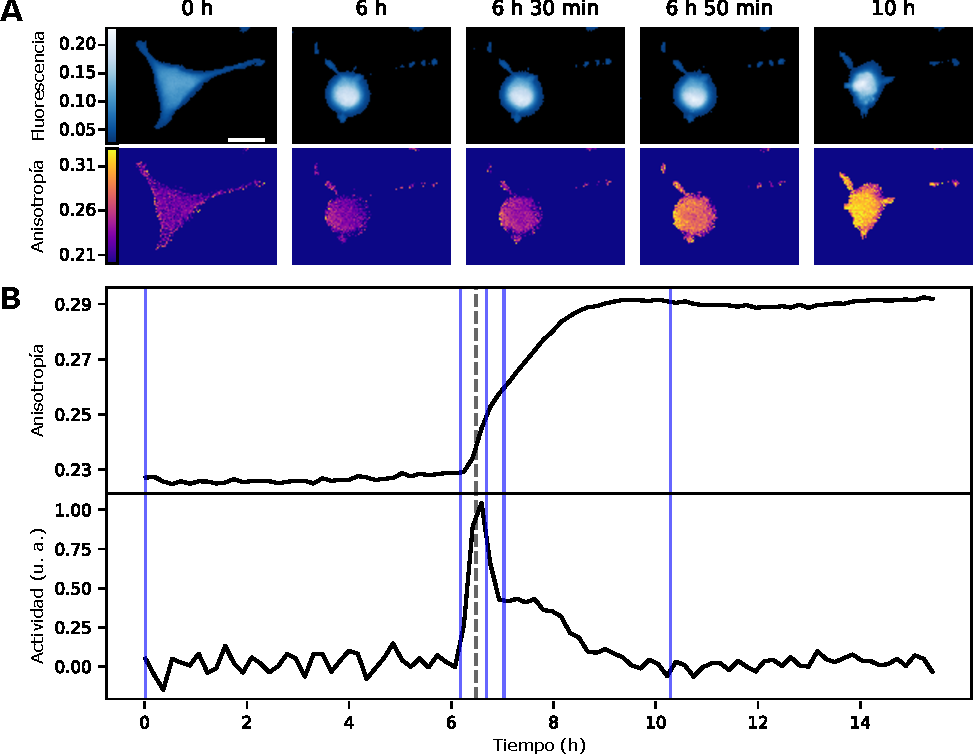
\includegraphics[width=0.9\textwidth]{img/cap_2/typical_derivation.pdf}
    \caption{\footnotesize{Análisis típico de una serie temporal de anisotropía. Adaptado de \cite{Corbat2018}. \textbf{A.} Imágenes de intensidad de fluorescencia y anisotropía correspondientes a una célula observada experimentalmente. Se puede apreciar como cambia la anisotropía a medida que la célula entra en apoptosis mientras que no varía fuertemente en intensidad. \textbf{B.} En el gráfico superior se muestra la anisotropía en función del tiempo de la célula analizada. Las líneas azules verticales corresponden a los tiempos de las imágenes mostradas en \textbf{A}. En el gráfico inferior se muestra la curva de actividad obtenida al analizar la curva de anisotropía.}}
    \label{fig:derivacion_tipica}
\end{figure}

Una vez generadas las curvas de actividad enzimática en función del tiempo, debemos definir un observable que sirva de referencia al momento en que se activaron las enzimas en estudio. Es común hallar en la bibliografía que se utilice el tiempo en el que algún porcentaje de biosensor es clivado (10\%, 50\% ó 90\%). Estos valores pueden determinarse mejor cuando la pendiente es elevada en los momentos alrededor del porcentaje de interés. 

Tratándose de perfiles de actividad enzimática, estos suelen seguir una forma sigmoidea o hiperbólica según las constantes cinéticas presentadas en la sección \ref{sec:CineticaEnzimatica}. Cuando el perfil de la curva tiene una forma sigmoidea, es fácil determinar el momento en que la mitad del biosensor es clivado, mientras que, si la curva tiene algo de ruido, se dificulta determinar el momento en que 10\% o 90\% del biosensor es clivado. Por otro lado, en los casos donde el perfil de clivaje es hiperbólico, esta mejor determinado el momento en que 10\% del sensor es clivado, en cambio el 90\% de clivaje tiene mucho error en su determinación.

Considerando que nuestro objetivo es obtener un tiempo que sirva de referencia de la activación de la enzima y que poseemos información de la actividad enzimática para todo tiempo, se evaluó utilizar el momento en el que se alcanza el máximo de actividad (\cref{fig:curvas_tipicas}). Determinarlo depende principalmente de la resolución temporal ya que sabemos con certeza que debe ubicarse entre los valores más elevados hallados. De esto se deriva la principal ventaja que es que dicha determinación puede ser utilizada sin importar el perfil de clivaje del biosensor. Además, dicho momento puede ser comparado fácilmente con simulaciones de la actividad enzimática. En búsqueda de mayor resolución temporal se utilizó una interpolación de bajo grado para hallarlo.

\begin{figure}[t!]
    \centering
    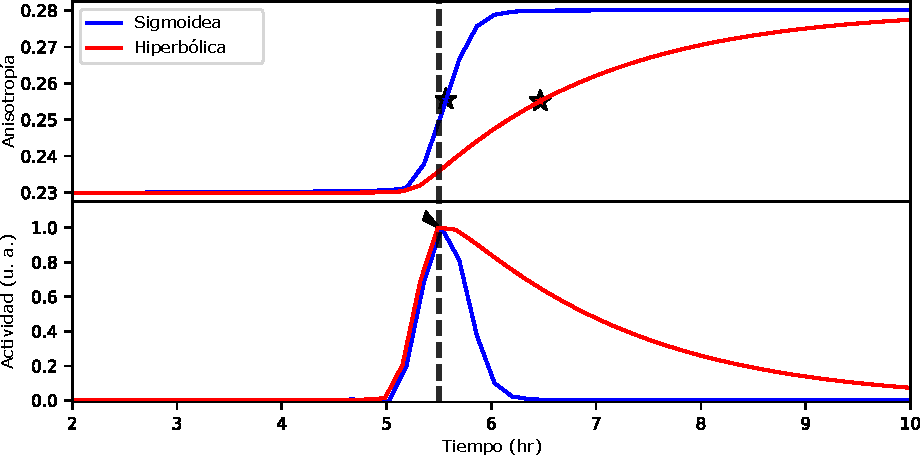
\includegraphics[width=0.9\textwidth]{img/cap_2/sim_analysis.pdf}
    \caption{\footnotesize{Se simularon dos perfiles de anisotropía típicos que se pueden hallar en experimentos con distintas enzimas: sigmoideo (azul) e hiperbólico (rojo). Las estrellas marcan el instante en el que se cliva 50\% del sensor y se puede apreciar que tiene distintas pendientes según la curva y ocurren en distintos momentos. La línea a trazos vertical marca el momento en el que se alcanza la máxima actividad de la enzima. Este momento es fácilmente determinado experimentalmente y puede ser relacionado fácilmente con las simulaciones. Adaptado de \cite{Corbat2018}.}}
    \label{fig:curvas_tipicas}
\end{figure}

En resumen, el flujo de análisis de datos comenzó con la adquisición del orden de cientos de imágenes por canal, entre las que se hallaron del orden de miles de células. Luego de procesar las imágenes, obtener las curvas de actividad para cada célula, se debió filtrar las curvas que correspondían a eventos apoptóticos y estimar el tiempo de máxima actividad de la caspasa en estudio. Cabe destacar que este flujo se puede caracterizar como de alto rendimiento al analizar miles de células, así como de reducción de datos ya que se obtiene un valor característico por cada curva.